\documentclass{beamer}

\usepackage{listings}
\usepackage{tabulary}
\usepackage{amsmath}
\usepackage[utf8]{inputenc}
\usetheme{Madrid}
\setbeamersize{text margin left=0.1\textwidth,text margin right=0.1\textwidth}
\setbeamertemplate{section in toc}{\inserttocsection}
\lstset{language=python,
        keywordstyle=\color{red},
        basicstyle=\ttfamily,
        basicstyle=\small,
        frame = single,
        framexleftmargin=15pt,
        numbers=left,
        numberstyle=\small,
        numbersep=5pt,
        xleftmargin=0.05\textwidth,
        columns=fullflexible}
\definecolor{dgreen}{rgb}{0.,0.6,0.}
\definecolor{goldenrod}{rgb}{.9,0.6,0.1}

%Information to be included in the title page:
\title{Matrix Factorization for Recommender Systems}
\author{Cary Goltermann}
\institute{Galvanize}
\date{2016}

\AtBeginSubsection[]
{
  \begin{frame}
    \frametitle{Overview}
    \tableofcontents[currentsection,currentsubsection]
  \end{frame}
}

\begin{document}

\frame{\titlepage}

\begin{frame}
  \frametitle{Overview}
  \tableofcontents[]
\end{frame}

\section{Matrix Factorzation Recommenders}
\subsection{Setup/Intuition}
\begin{frame}
  \frametitle{Setup $\rightarrow$ Sparse Ratings Matrix}
  \begin{center}
  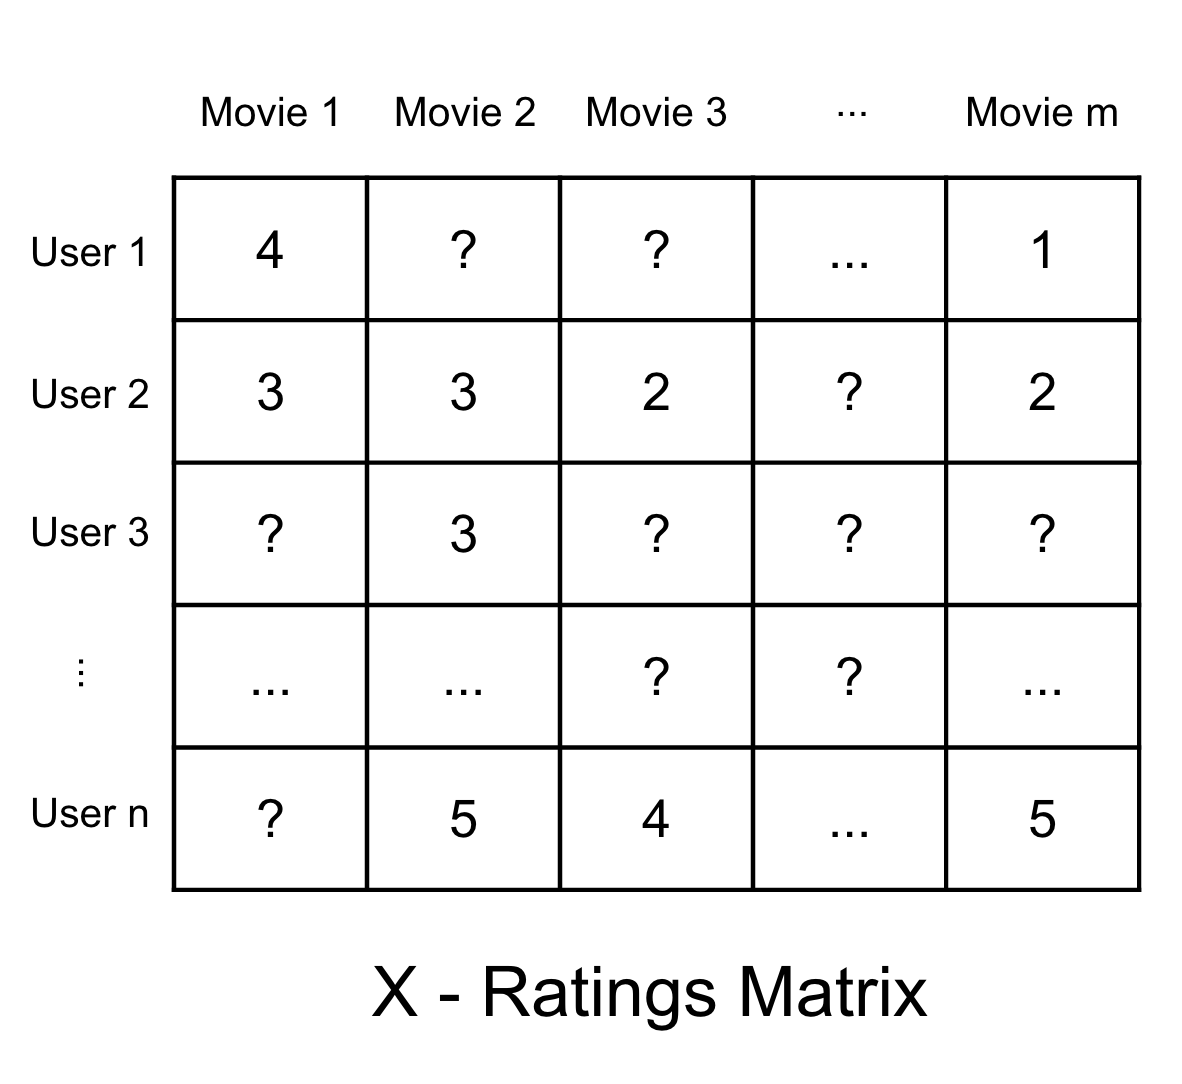
\includegraphics[width=0.6\textwidth]{images/ratings_matrix.png}
  \end{center}
  Could be very, very sparse $\rightarrow 99\% $ of entries unknown.
\end{frame}

\begin{frame}
  \frametitle{Downfall of Collaborative Filtering}
  \begin{description}
    \item[Item-Item] I like action movies $\rightarrow$ rate \textit{Top Gun} and \textit{Mission Impossible} 5s. \par $\rightarrow$ I'm recommended \textit{Jerry Maguire} even though I won't like it. \vspace{4mm}
    \item[User-User] I like Tom Cruise $\rightarrow$ rate \textit{Top Gun} and \textit{Mission Impossible} 5s. \par $\rightarrow$ I'm recommended \textit{Transformers} even though I won't like it.
  \end{description}
\end{frame}

\begin{frame}
  \frametitle{Movies (and Everything Else) Have Attributes}
  \begin{itemize}
    \item Action, Romance, Comedy, etc.
    \item Tom Criuse, Tom Hanks, Megan Fox, etc.
    \item Long, Short, Subtitles, Foreign, Happy, Sad, etc.
  \end{itemize}
\end{frame}

\begin{frame}
  \frametitle{Could We Use a Linear Regression?}
  \begin{align*}
    Rating\; Prediction = \beta_0 &+ \beta_1 \times actionness + ... \\
    &+ \beta_i \times foxiness + ... \\
    &+ \beta_j \times sadness + \epsilon
  \end{align*} \vspace{4mm} \pause

  Possibly...though we'd have to come up with some measure of actionness, etc. This is both subject to error and rather brittle.
\end{frame}

\subsection{Factorization}
\begin{frame}
  \frametitle{What About Factorization?}
  \begin{itemize}
    \item Factorization could account for something along the lines of these attributes as was our hope in LR. \vspace{2mm}
    \item All of the factorization models that we know can be interpreted as a linear combination of bases. \vspace{2mm}
    \item There's a chance, especially with NMF, that those bases, latent features, could correspond with some of these ``attributes'' that we're looking to describe the movies with.
  \end{itemize}
\end{frame}

\begin{frame}
  \frametitle{Factorization Problem}
  \begin{itemize}
    \item \textbf{Problem:} PCA, SVD and NMF \textbf{all} must be computed on a \textbf{dense} data matrix, $X$. \vspace{2mm}
    \item Potential Soluation: inpute missing values, naively, with something like the mean of the known values. \textit{Note: This is what sklearn does when it says it factorizes sparse matrices.}
  \end{itemize}
\end{frame}

\begin{frame}
  \frametitle{Factorization Goal}
  \begin{itemize}
    \item Create a factorization for a sparse data matrix, $X$, into $U \cdot V$, such that the reconstruction to $\hat{X}$ serves as a model. \vspace{2mm}
    \item More formally, for a previously unknown entry in $X$, $X_{i,j}$ the corresponding entry in $\hat{X}$, $\hat{X}_{i,j}$ serves as a prediction. \vspace{2mm}
    \item \textit{Note: Since we could easily overfit the known values in $X$ we want to regularize, one way to do this is by reducing the inner dimension in $U$ and $V$, $k$.}
  \end{itemize}
\end{frame}

\begin{frame}
  \frametitle{Factorization Visual}
  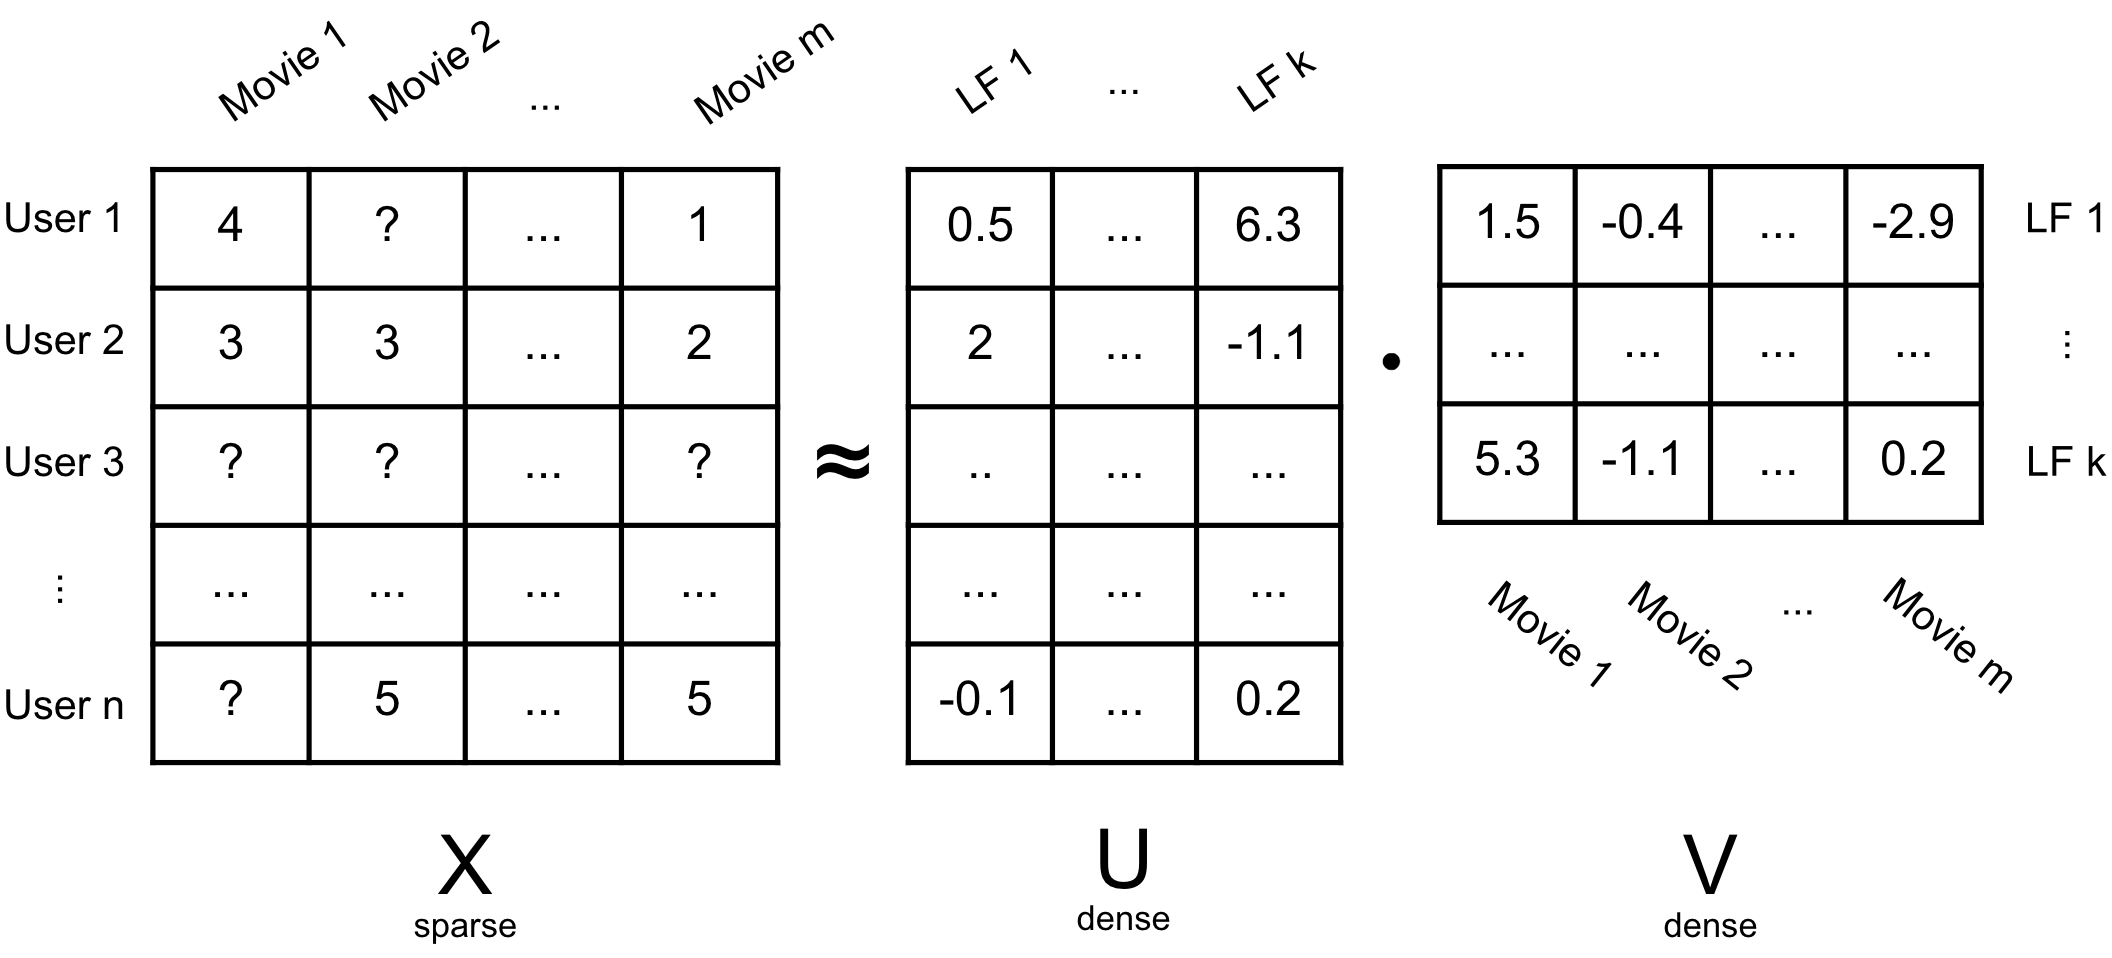
\includegraphics[width=\textwidth]{images/factorization.png} \vspace{4mm}
\end{frame}

\begin{frame}
  \frametitle{Reconstruction Visual}
  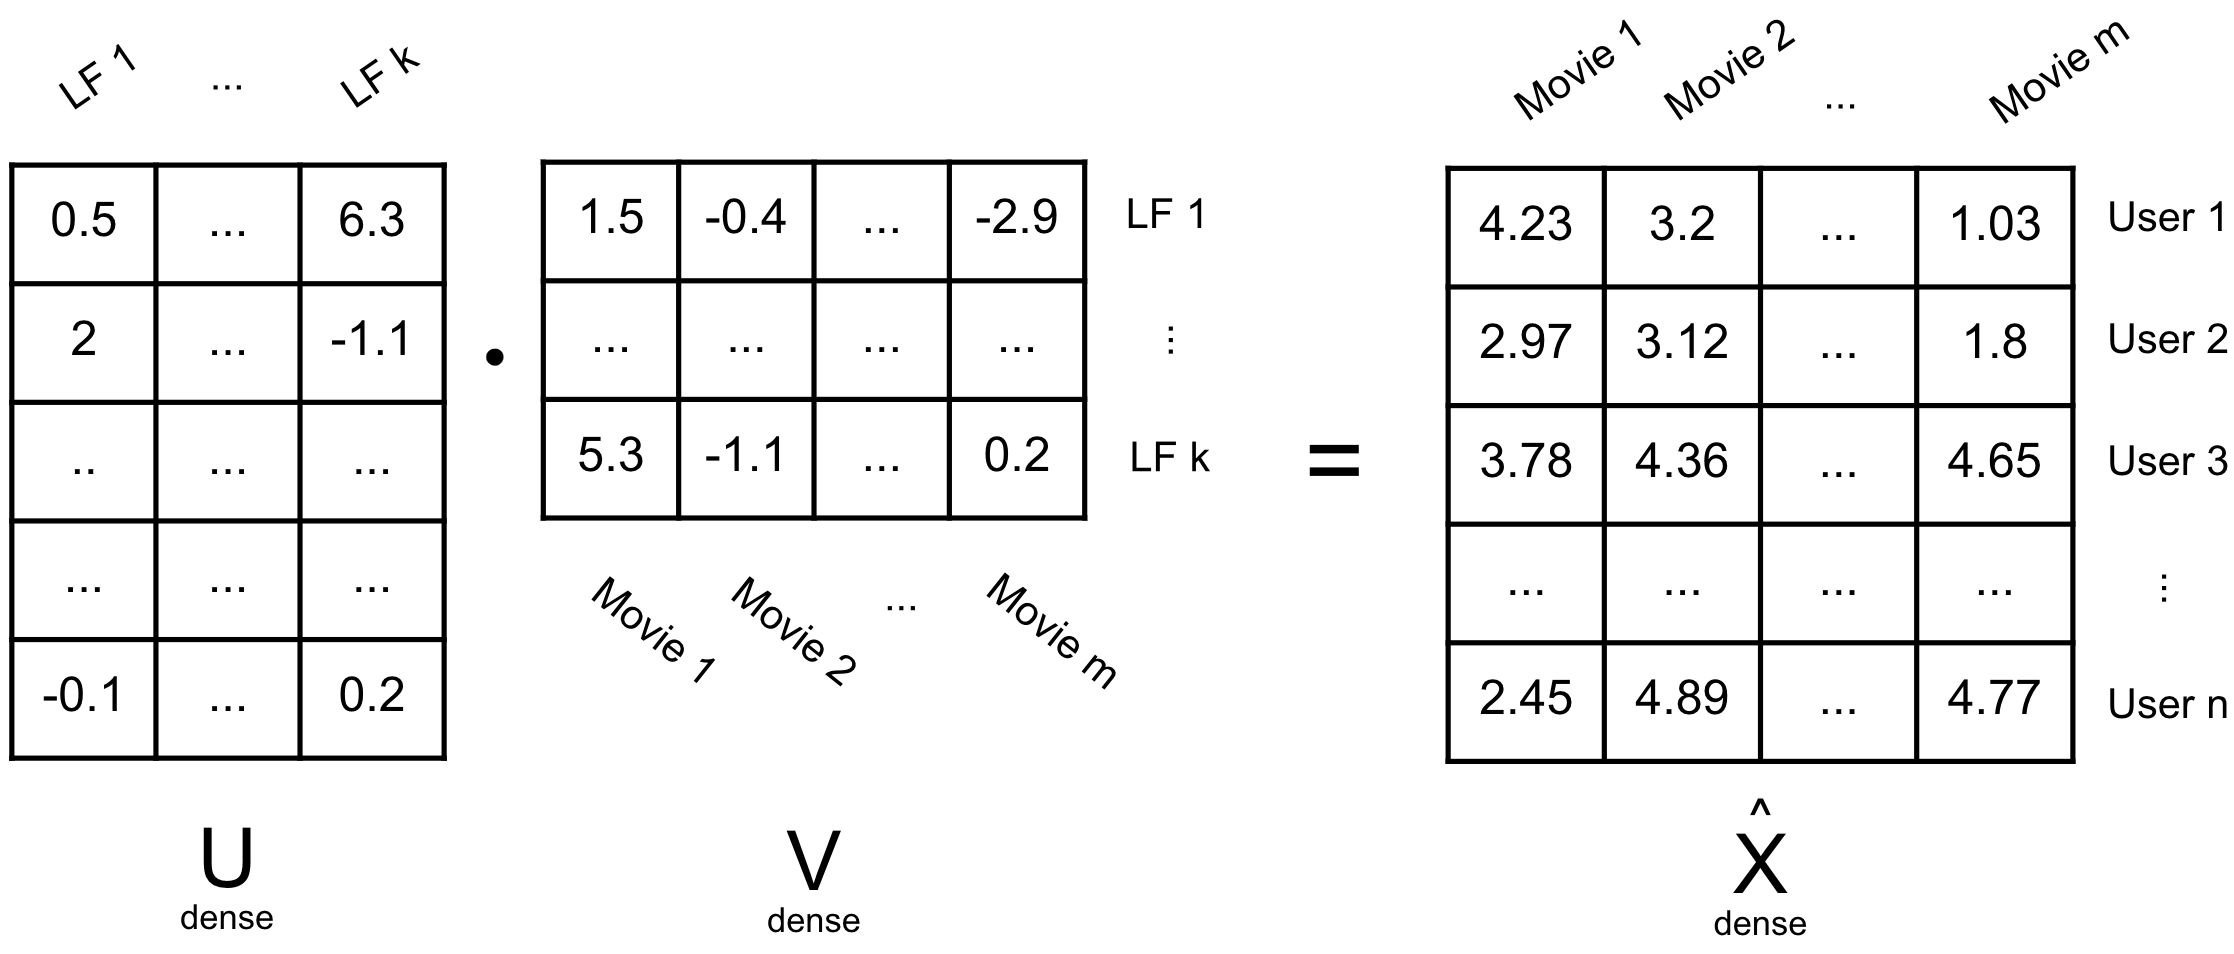
\includegraphics[width=\textwidth]{images/reconstruction.png} \vspace{4mm}
\end{frame}

\begin{frame}
  \frametitle{Difference between CF and MF}
  \begin{itemize}
    \item Collaborative Filtering (neighborhood models) $\rightarrow$ \textbf{Memory Based}. Just store data so we can query what/whom is most similar when asked to recommend. \vspace{2mm}
    \item Factorization Techniques $\rightarrow$ \textbf{Model Based}. Creates predictions, from which the most suitable can be recommended.
  \end{itemize}
\end{frame}

\begin{frame}
  \frametitle{Computing the Factorization}
  \begin{itemize}
    \item Similar to what we did to find the factorization in NMF, we're going to minimize a cost function. \vspace{2mm}
    \item Now, though we can't do it at the level of the entirety of $X$, since it is sparse. \vspace{2mm}
    \item However, we can optimize with respect to the data in $X$ that we do have.
  \end{itemize}
\end{frame}

\begin{frame}
  \frametitle{Factorization Plan}
    For each of the known ratings in $X_{i,j}$ we want to minimize the square error in the prediction that results from $U_i \cdot V_j$, a.k.a. 

    $$ \underset{U,V}{min} \sum\limits_{(i,j) \in K} (X_{i,j} - U_i \cdot V_j)^2. $$
    
    Where $U_i$ is the $i^{th}$ row of $U$, $V_j$ is the $j^{th}$ column of $V$, and $K$ is the set of indices in $X$ that have data.
\end{frame}

\begin{frame}
  \frametitle{Reconstructing a Single Entry}
  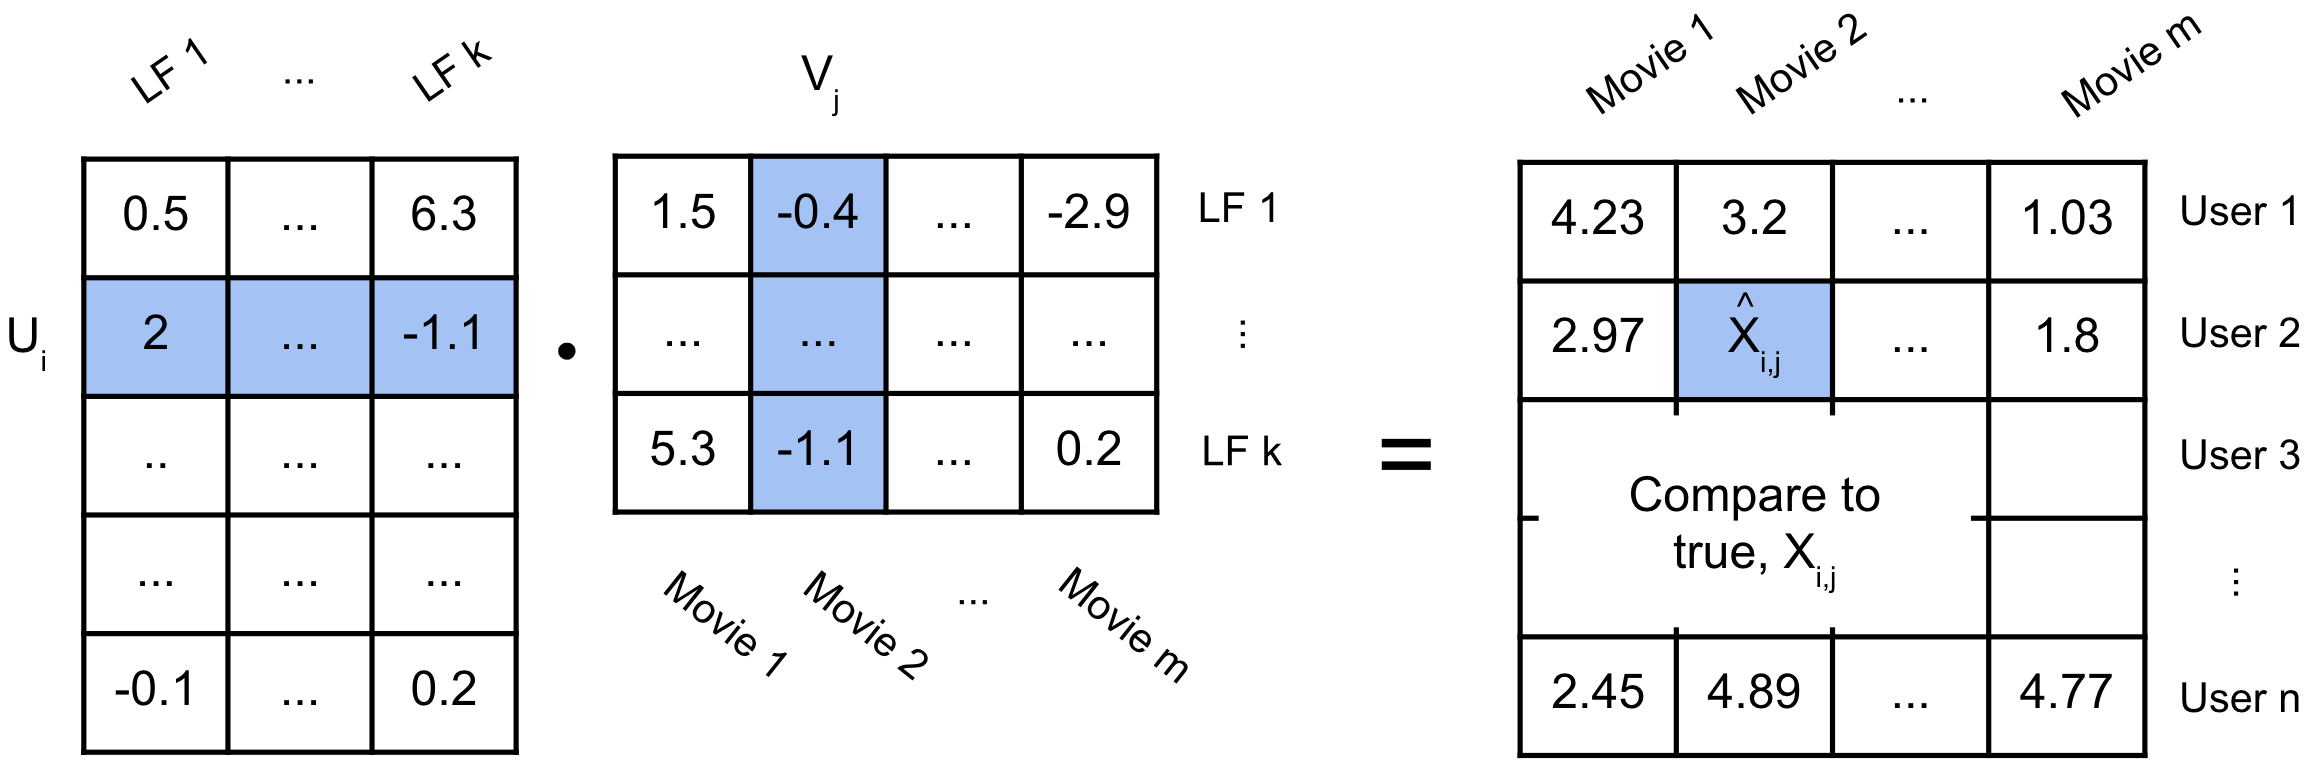
\includegraphics[width=\textwidth]{images/reconstruction_cell.png} \vspace{4mm}
\end{frame}

\subsection{Algorithms}
\begin{frame}
  \frametitle{Algorithms}
  \begin{itemize}
    \item This minimization can be solved with ALS, rotating between fixing the $U_i$s to solve for the $V_j$s and fixing the $V_j$s to solve for the $U_i$s. \vspace{4mm}
    \item A more popular alternative is a version of gradient descent popularized by Simon Funk during the Netflix prize, know as Funk SVD.
  \end{itemize}
\end{frame}

\begin{frame}
  \frametitle{Funk SVD}
  \begin{itemize}
    \item Define the error on a particular prediction in $X$ as $e_{i,j} = X_{i,j} - \hat{X}_{i,j}$. \vspace{4mm}
    \item Then we can update the columns in $U$ and $V$ with:
    \begin{itemize}
      \item $U_i \leftarrow U_i + \nu(e_{i,j}V_j)$
      \item $V_j \leftarrow V_j + \nu(e_{i,j}U_i)$
    \end{itemize}
  \end{itemize}
\end{frame}

\begin{frame}
  \frametitle{Funk SVD Algorithm}
  Initialize $U$ and $V$ with small random values. \vspace{1mm}

  While error is decreasing:
  \begin{itemize}
    \item For each user, $i$:
    \begin{itemize}
      \item For each item rated by that user, $j$:
      \begin{enumerate}
        \item Predict rating, $\hat{X}_{i,j}$.
        \item Calculate $e_{i,j}$.
        \item Update $U_i$ and $V_j$.
      \end{enumerate}
    \end{itemize}
  \end{itemize}
\end{frame}

\subsection{Nuances}
\begin{frame}
  \frametitle{Baseline Predictors (Biases)}
  \begin{itemize}
    \item Much of the observed ratings are associated with a specific user's personality or an item's intrinsic value, not an interaction between the two which is what get captured in the factorization.
    \item To encapsulate these effects, which do not involve user-item interactions, we introduce \textbf{baseline predictors}.
    \begin{itemize}
      \item $\mu$: Baseline average value in $X$.
      \item $b_i$: Baseline rating for user $i$.
      \item $b_j$: Baseline rating for item $j$.
    \end{itemize}
    \item From this we can describe our predictions with: 
      $$ \hat{X}_{i,j} = \mu + b_i + b_j + U_i \cdot V_j. $$
  \end{itemize}
\end{frame}

\begin{frame}
  \frametitle{Regularization}
  \begin{itemize}
    \item Another way to regularize our decomposition to help prevent from overfitting to our sparse data is via a penalty, $\lambda$, placed on the magnitude of: $b_i$, $b_j$, $U_i$ and $V_j$. The most common is the $L_2$ norm. \vspace{2mm}
    \item Such a penalty changes our cost function to:
      $$ \underset{b_:, U,V}{min} \sum\limits_{(i,j) \in K} (X_{i,j} - U_i \cdot V_j)^2 + \lambda(b_i^2 + b_j^2 + \vert U_i \vert^2 + \vert V_j \vert^2)$$
  \end{itemize}
\end{frame}

\begin{frame}
  \frametitle{Regularization Update Rules}
  With these considerations the update rules become:

  \begin{columns}
    \column{0.6\textwidth}
    \begin{itemize}
      \item $b_i \leftarrow b_i + \nu(e_{i,j} - \lambda b_i)$
      \item $b_j \leftarrow b_j + \nu(e_{i,j} - \lambda b_j)$
      \item $U_i \leftarrow U_i + \nu(e_{i,j}V_j - \lambda U_i)$
      \item $V_j \leftarrow V_j + \nu(e_{i,j}U_i - \lambda V_j)$
    \end{itemize}
  \end{columns}
\end{frame}

\subsection{Final Thoughts}
\begin{frame}
  \frametitle{Validation}
  Validating any recommender is difficult, but it is necessary as we're going to want to tune the hyperparameters that we introduced into our model, $\nu$ and $\lambda$. \vspace{2mm}
  
  The most frequently used metric is Root Mean Squared Error (RMSE) on the known data:

  $$ RMSE = \sqrt{\sum\limits_{(1,j) \in K} (X_{i,j} - \hat{X}_{i,j})^2} $$
\end{frame}

\begin{frame}
  \frametitle{MF - Pros/Cons}
  \begin{columns}
    \column{0.5\textwidth}
    \begin{center} {\LARGE \textcolor{blue}{Pros}} \end{center}
    \column{0.5\textwidth}
    \begin{center} {\LARGE \textcolor{blue}{Cons}} \end{center}
  \end{columns} \vspace{4mm}
  \begin{columns}
    \column[T]{0.5\textwidth}
    \begin{itemize}
      \item Decent with sparsity, so long as we regularize.
      \item Prediction is fast, only need to do an inner product.
      \item Can inspect latent features for topical meaning.
      \item Can be extended to include side information.
    \end{itemize}
    \column[T]{0.5\textwidth}
    \begin{itemize}
      \item Need to re-factorize with new data. Very slow.
      \item Fails in the cold start case.
      \item Not great open source tools for huge matrices.
      \item Difficult to tune directly to the type of recommendation you want to make. Tied to the difficulty of measuring success.
    \end{itemize}
  \end{columns}
\end{frame}

\begin{frame}
  \frametitle{Advanced Factorization Methods}
  \begin{itemize}
    \item Non-negativity constraint $\rightarrow$ More interpretable latent features. \vspace{2mm} 
    \item SVD++ $\rightarrow$ uses implicit feedback (clicks, likes, etc.) to enhance model. \vspace{2mm}
      \item Time-aware factor model $\rightarrow$ accounts for temporal information about data.
  \end{itemize}
\end{frame}

\end{document}
